\section*{Results}

\subsection*{Dataset and evaluation}

We assembled a nucleotide-encoded SNP feature matrix from 9{,}798 publicly available \emph{M. tuberculosis} isolates, comprising 2{,}693 positions across nine genes associated with resistance to the four first-line drugs (Methods; Fig.~\ref{fig:pipeline}). Phenotypic label availability differs by drug, reflecting which isolates were tested against which agent in the source studies: 9{,}630 isolates for rifampicin, 9{,}580 for isoniazid, 8{,}196 for ethambutol, and 5{,}749 for pyrazinamide (Table~\ref{tab:dataset}). Class balance also varies substantially, from near-parity for ethambutol (49.8\% resistant) and pyrazinamide (45.4\% resistant) to strongly resistant-skewed for isoniazid (86.0\% resistant). All models were evaluated on an 80/20 stratified train/test split with 5-fold stratified cross-validation on the training partition, reporting accuracy and AUC-ROC; the multi-label formulation was additionally assessed by Hamming loss and subset (exact-match) accuracy.

\begin{table}[h]
\centering
\caption{Dataset summary. Isolates and per-drug phenotype label counts after quality-control filtering (3 outliers removed: ERR1034652, ERR1035353, ERR1213920).}
\label{tab:dataset}
\begin{tabular}{lrrr}
\toprule
Drug & Labelled isolates & Resistant, n (\%) & Susceptible, n (\%) \\
\midrule
Rifampicin   & 9{,}630 & 7{,}144 (74.2\%) & 2{,}486 (25.8\%) \\
Isoniazid    & 9{,}580 & 8{,}238 (86.0\%) & 1{,}342 (14.0\%) \\
Ethambutol   & 8{,}196 & 4{,}082 (49.8\%) & 4{,}114 (50.2\%) \\
Pyrazinamide & 5{,}749 & 2{,}610 (45.4\%) & 3{,}139 (54.6\%) \\
\bottomrule
\end{tabular}

\vspace{4pt}
\footnotesize
Total isolates in the final feature matrix: 9{,}798. Feature count: 2{,}693 nucleotide-encoded SNP positions across nine AMR genes (\emph{rpoB}; \emph{katG}, \emph{inhA}, \emph{fabG1}; \emph{embB}, \emph{embA}, \emph{embC}; \emph{pncA}, \emph{rpsA}). The underlying phenotype table covers 23{,}051 isolates across 23 drugs; only the four first-line drugs above are modelled here.
\end{table}


\subsection*{Per-drug classifier performance}

Across all four first-line drugs, Random Forest achieved the highest cross-validated AUC-ROC among the seven benchmarked classifiers (Table~\ref{tab:modelcomparison}), and its final per-drug models achieved test-set AUC-ROC of 0.976 (rifampicin), 0.947 (isoniazid), 0.894 (ethambutol), and 0.886 (pyrazinamide), with corresponding 5-fold CV AUC-ROC of 0.969, 0.946, 0.900, and 0.883 (Table~\ref{tab:perdrug}). Gradient-boosted alternatives (LightGBM, XGBoost) tracked Random Forest closely on rifampicin and isoniazid but fell further behind on ethambutol and pyrazinamide; the linear SVM trained via SGD was the weakest model on every drug, most markedly on ethambutol (CV AUC-ROC 0.780 vs. 0.900 for Random Forest). Performance ordering across drugs (rifampicin~$>$~isoniazid~$>$~ethambutol~$\approx$~pyrazinamide) was consistent between the per-drug models (Table~\ref{tab:perdrug}) and the independent multi-model benchmarking run (Table~\ref{tab:modelcomparison}).

\begin{table}[h]
\centering
\caption{Per-drug Random Forest classifier performance (final v2 models; 80/20 stratified train/test split, 300 trees, \texttt{class\_weight="balanced"}). CV columns report 5-fold stratified cross-validation, mean $\pm$ SD.}
\label{tab:perdrug}
\begin{tabular}{lrrrr}
\toprule
Drug & Test Acc. & Test AUC-ROC & CV Acc. & CV AUC-ROC \\
\midrule
Rifampicin   & 0.9496 & 0.9759 & 0.9366 $\pm$ 0.0040 & 0.9688 $\pm$ 0.0039 \\
Isoniazid    & 0.9045 & 0.9473 & 0.9056 $\pm$ 0.0037 & 0.9462 $\pm$ 0.0074 \\
Ethambutol   & 0.8091 & 0.8936 & 0.8208 $\pm$ 0.0048 & 0.8996 $\pm$ 0.0066 \\
Pyrazinamide & 0.8200 & 0.8862 & 0.8116 $\pm$ 0.0133 & 0.8831 $\pm$ 0.0075 \\
\bottomrule
\end{tabular}

\vspace{4pt}
\footnotesize
Per-class precision/recall/F1 (test split): Rifampicin -- Susceptible 0.86/0.95/0.91, Resistant 0.98/0.95/0.97 ($n=1{,}926$); Isoniazid -- Susceptible 0.61/0.91/0.73, Resistant 0.98/0.90/0.94 ($n=1{,}916$); Ethambutol -- Susceptible 0.78/0.86/0.82, Resistant 0.84/0.76/0.80 ($n=1{,}640$); Pyrazinamide -- Susceptible 0.80/0.89/0.84, Resistant 0.85/0.74/0.79 ($n=1{,}150$).
\end{table}

\begin{table}[h]
\centering
\caption{Seven-model benchmark, 5-fold stratified cross-validation AUC-ROC per drug (independent benchmarking run from the per-drug models in Table~\ref{tab:perdrug}; minor numeric differences between the two tables reflect independent train/test splits, not a discrepancy). Bold marks the best CV AUC-ROC per drug.}
\label{tab:modelcomparison}
\small
\begin{tabular}{lrrrr}
\toprule
Model & Rifampicin & Isoniazid & Ethambutol & Pyrazinamide \\
\midrule
Random Forest        & \textbf{0.9690} & \textbf{0.9464} & \textbf{0.8997} & \textbf{0.8831} \\
LightGBM              & 0.9675 & 0.9391 & 0.8938 & 0.8699 \\
XGBoost                & 0.9643 & 0.9364 & 0.8840 & 0.8595 \\
LR L1 (Lasso)          & 0.9607 & 0.9433 & 0.8696 & 0.8660 \\
LR ElasticNet          & 0.9602 & 0.9428 & 0.8651 & 0.8614 \\
LR L2 (Ridge)          & 0.9568 & 0.9382 & 0.8569 & 0.8488 \\
Linear SVM (SGD)       & 0.9155 & 0.8782 & 0.7796 & 0.7912 \\
\bottomrule
\end{tabular}

\vspace{4pt}
\footnotesize
Same 80/20 train/test split and 5-fold stratified CV protocol as Table~\ref{tab:perdrug}, run independently per model family.
\end{table}


\subsection*{SHAP-based interpretability}

SHAP summary plots for the four per-drug Random Forest models (Figure~\ref{fig:shap_summary}) show that the top-ranked feature for rifampicin and isoniazid corresponds to a single dominant genomic position each, consistent with the well-characterized resistance mutations \emph{rpoB} S450L and \emph{katG} S315T, respectively. For ethambutol, attribution is more distributed across multiple \emph{embB} positions, consistent with the polygenic and comparatively lower discriminative performance observed in Table~\ref{tab:perdrug}. These associations were not supplied to the model as prior knowledge; they emerge purely from feature importance on the encoded SNP matrix, providing a form of internal validation that the classifiers are learning biologically plausible signal rather than confounded artefacts.

\begin{figure}[h]
\centering
\begin{minipage}{0.48\textwidth}
\centering
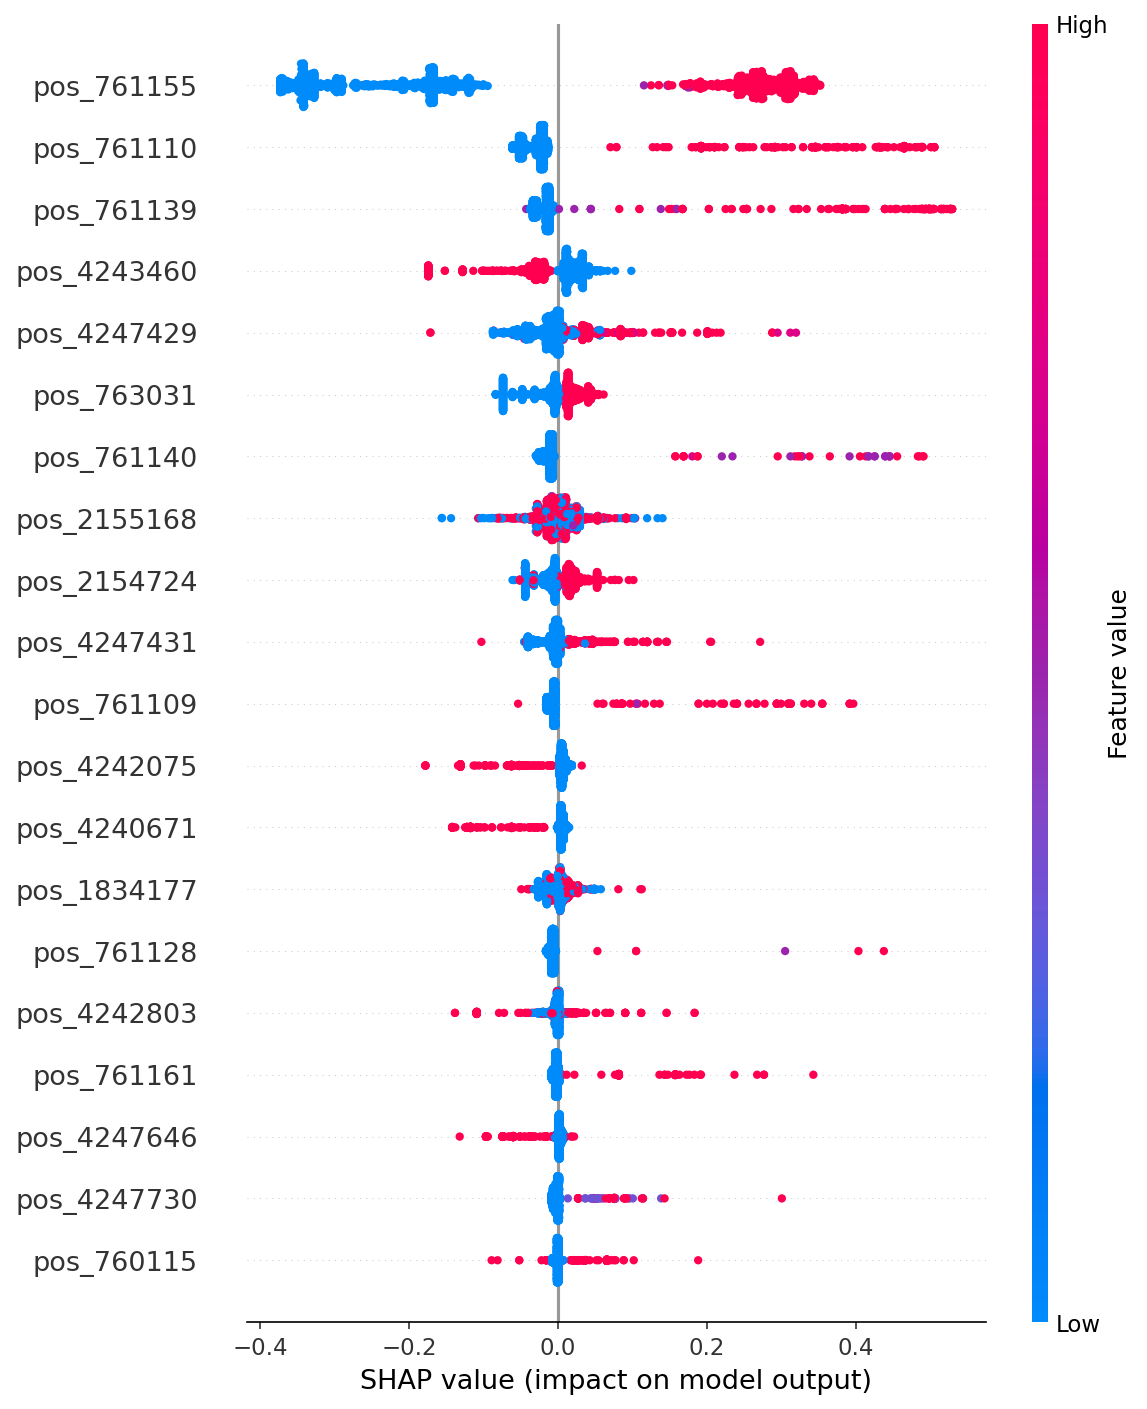
\includegraphics[width=\linewidth]{figures/fig2a_shap_rifampicin.png}
\caption*{(a) Rifampicin}
\end{minipage}
\hfill
\begin{minipage}{0.48\textwidth}
\centering
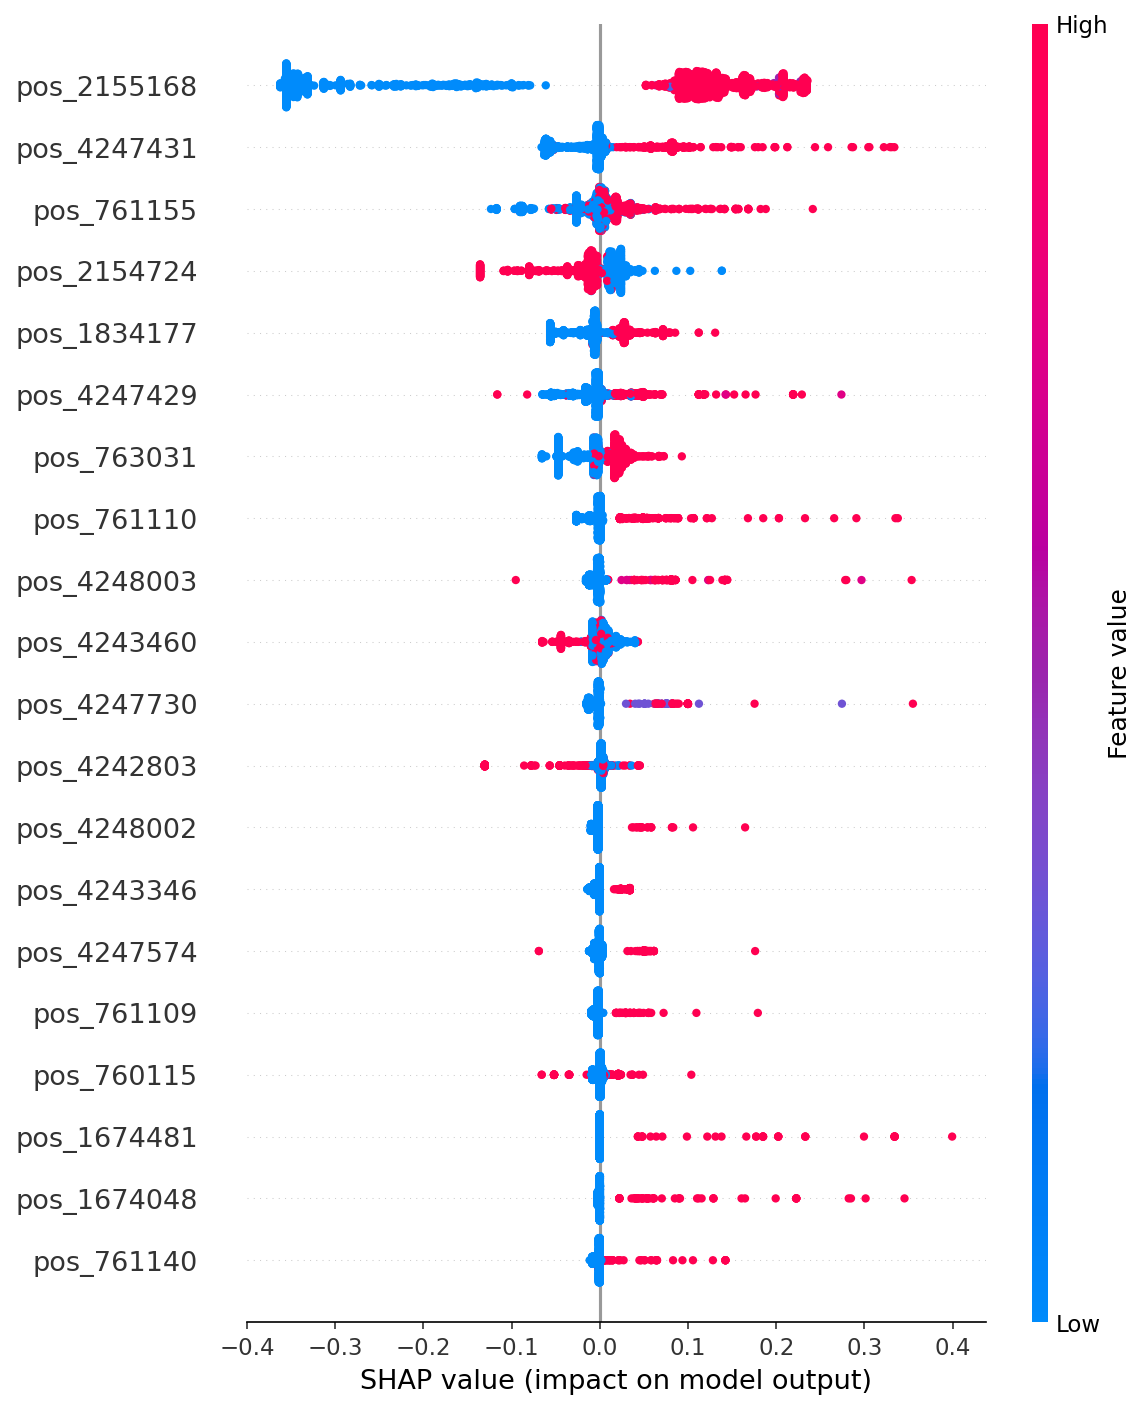
\includegraphics[width=\linewidth]{figures/fig2b_shap_isoniazid.png}
\caption*{(b) Isoniazid}
\end{minipage}

\vspace{6pt}
\begin{minipage}{0.48\textwidth}
\centering
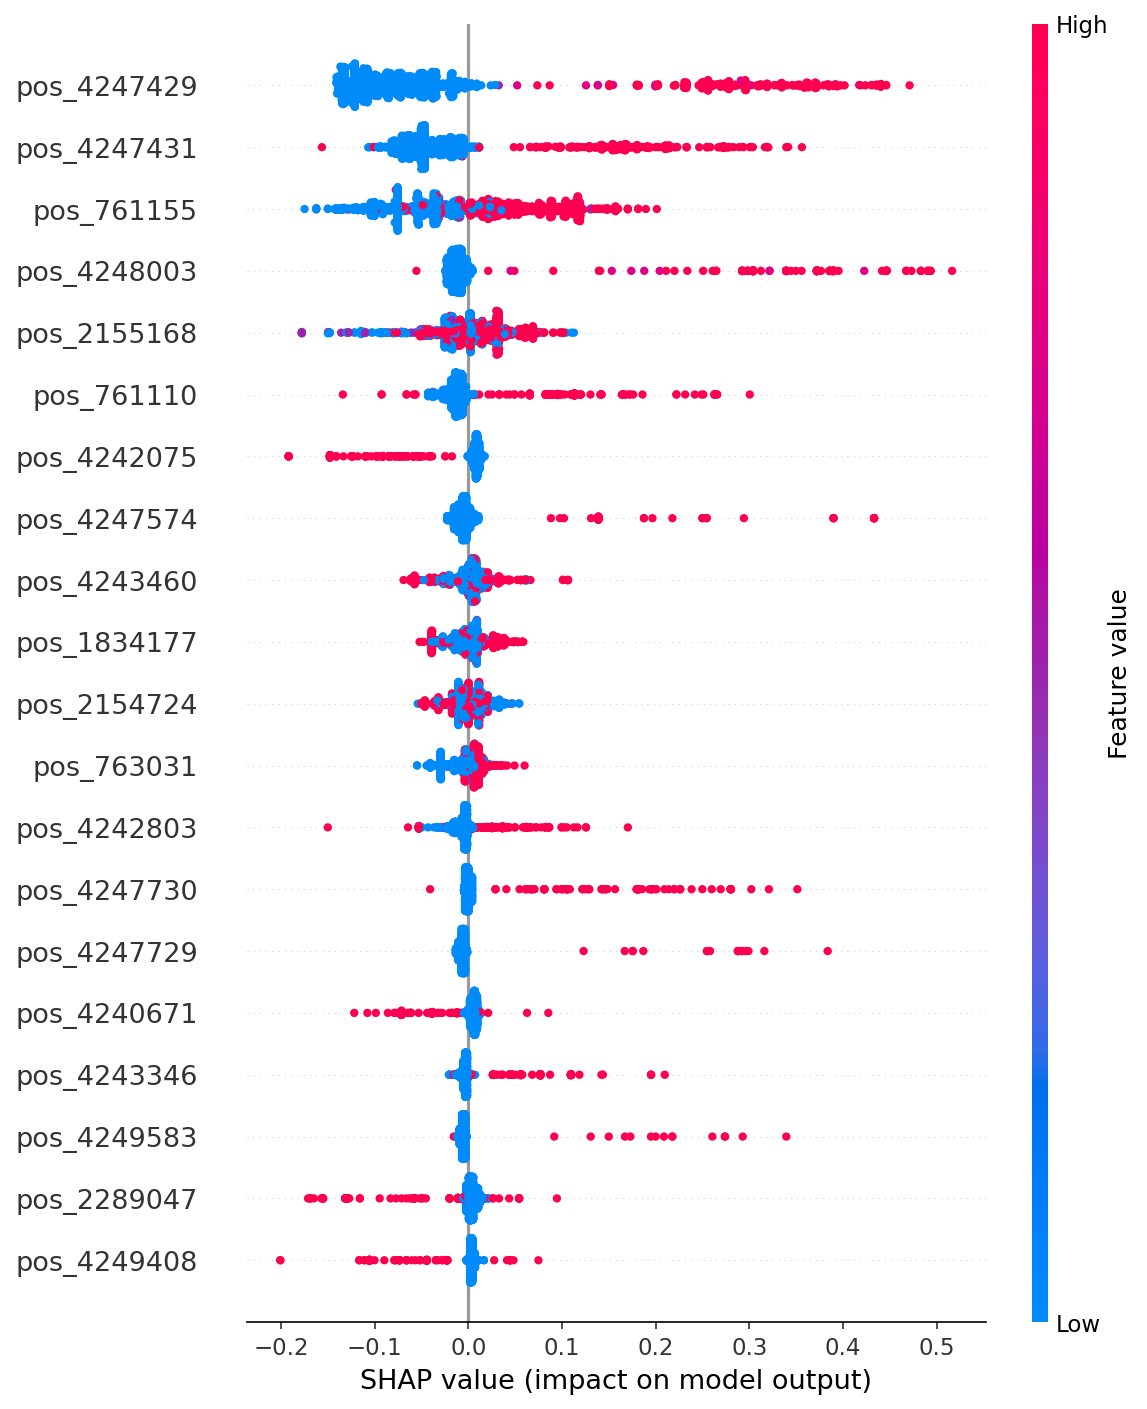
\includegraphics[width=\linewidth]{figures/fig2c_shap_ethambutol.png}
\caption*{(c) Ethambutol}
\end{minipage}
\hfill
\begin{minipage}{0.48\textwidth}
\centering
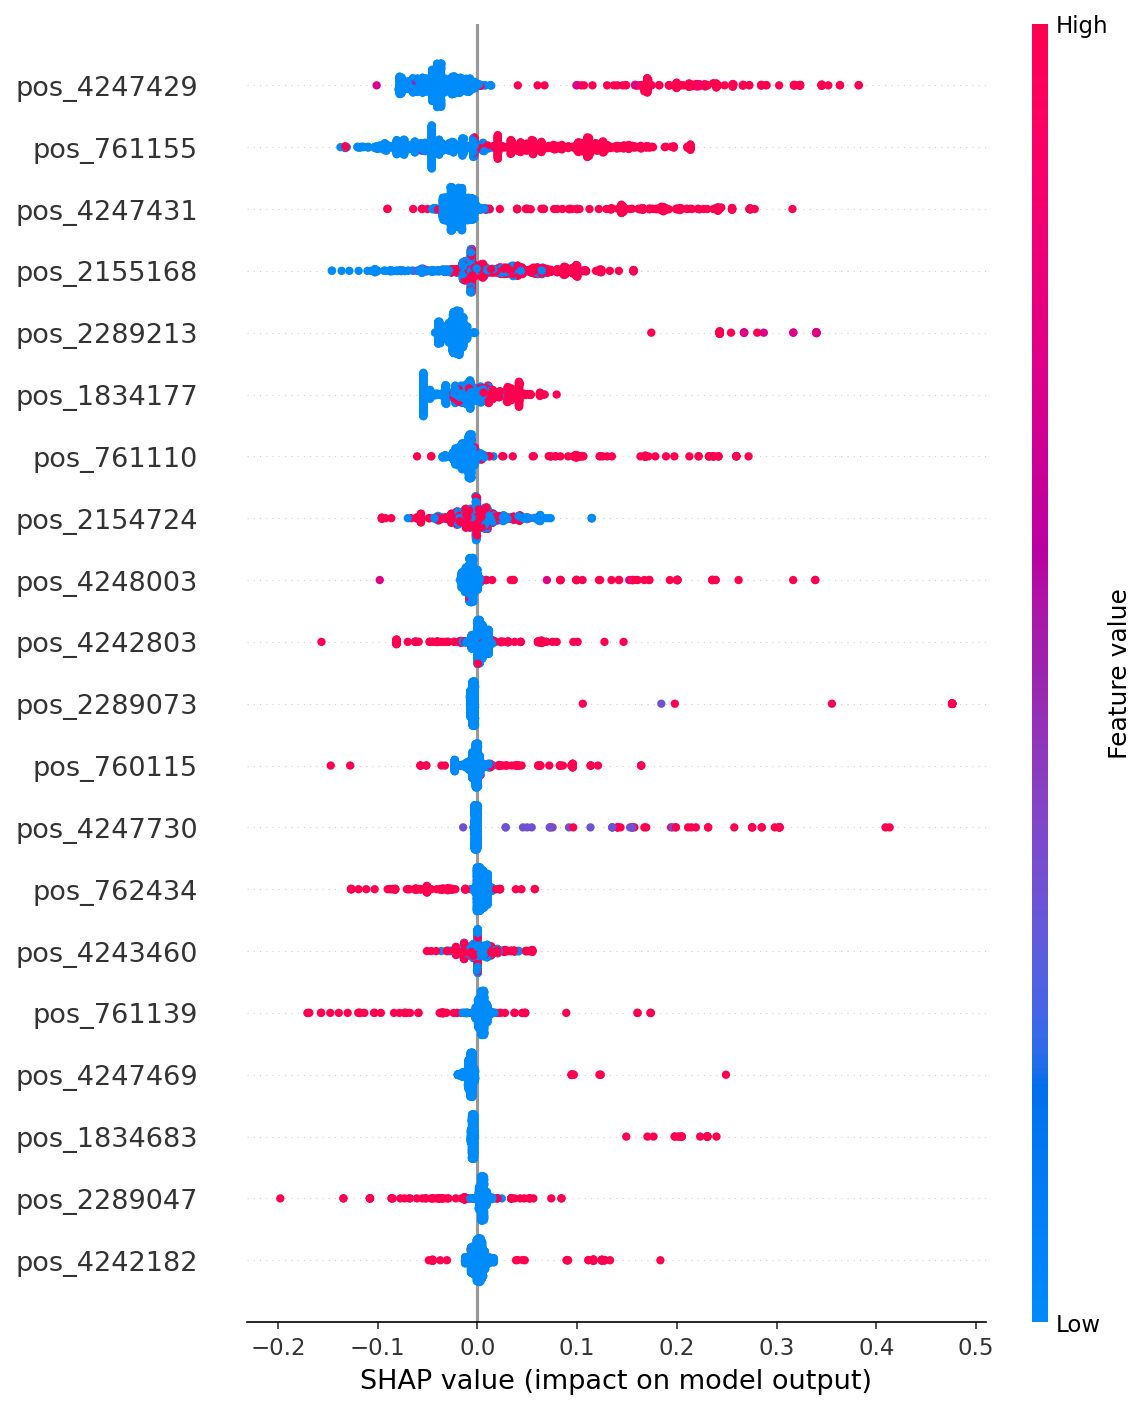
\includegraphics[width=\linewidth]{figures/fig2d_shap_pyrazinamide.png}
\caption*{(d) Pyrazinamide}
\end{minipage}
\caption{SHAP summary (beeswarm) plots for the top-50-feature Random Forest model, one panel per drug. Each point is one isolate; horizontal position is the SHAP value (contribution to predicted resistance log-odds), color encodes the encoded nucleotide value, and features are ranked top-to-bottom by mean absolute SHAP value.}
\label{fig:shap_summary}
\end{figure}

\begin{figure}[h]
\centering
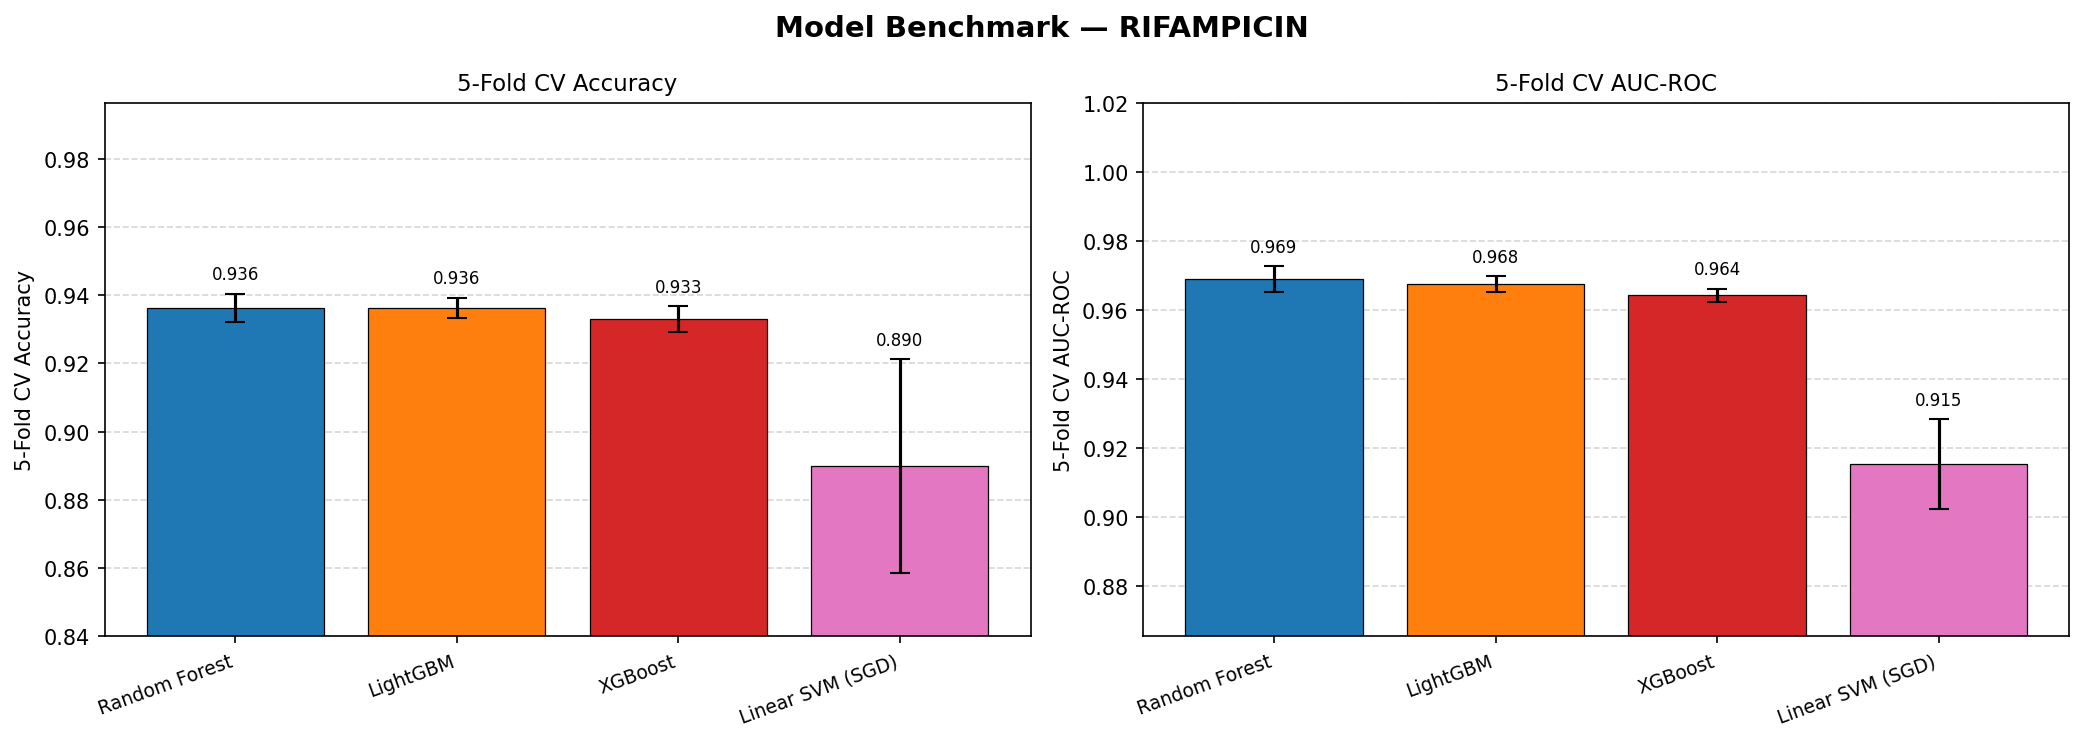
\includegraphics[width=0.85\linewidth]{figures/fig3a_benchmark_rifampicin.png}
\vspace{4pt}
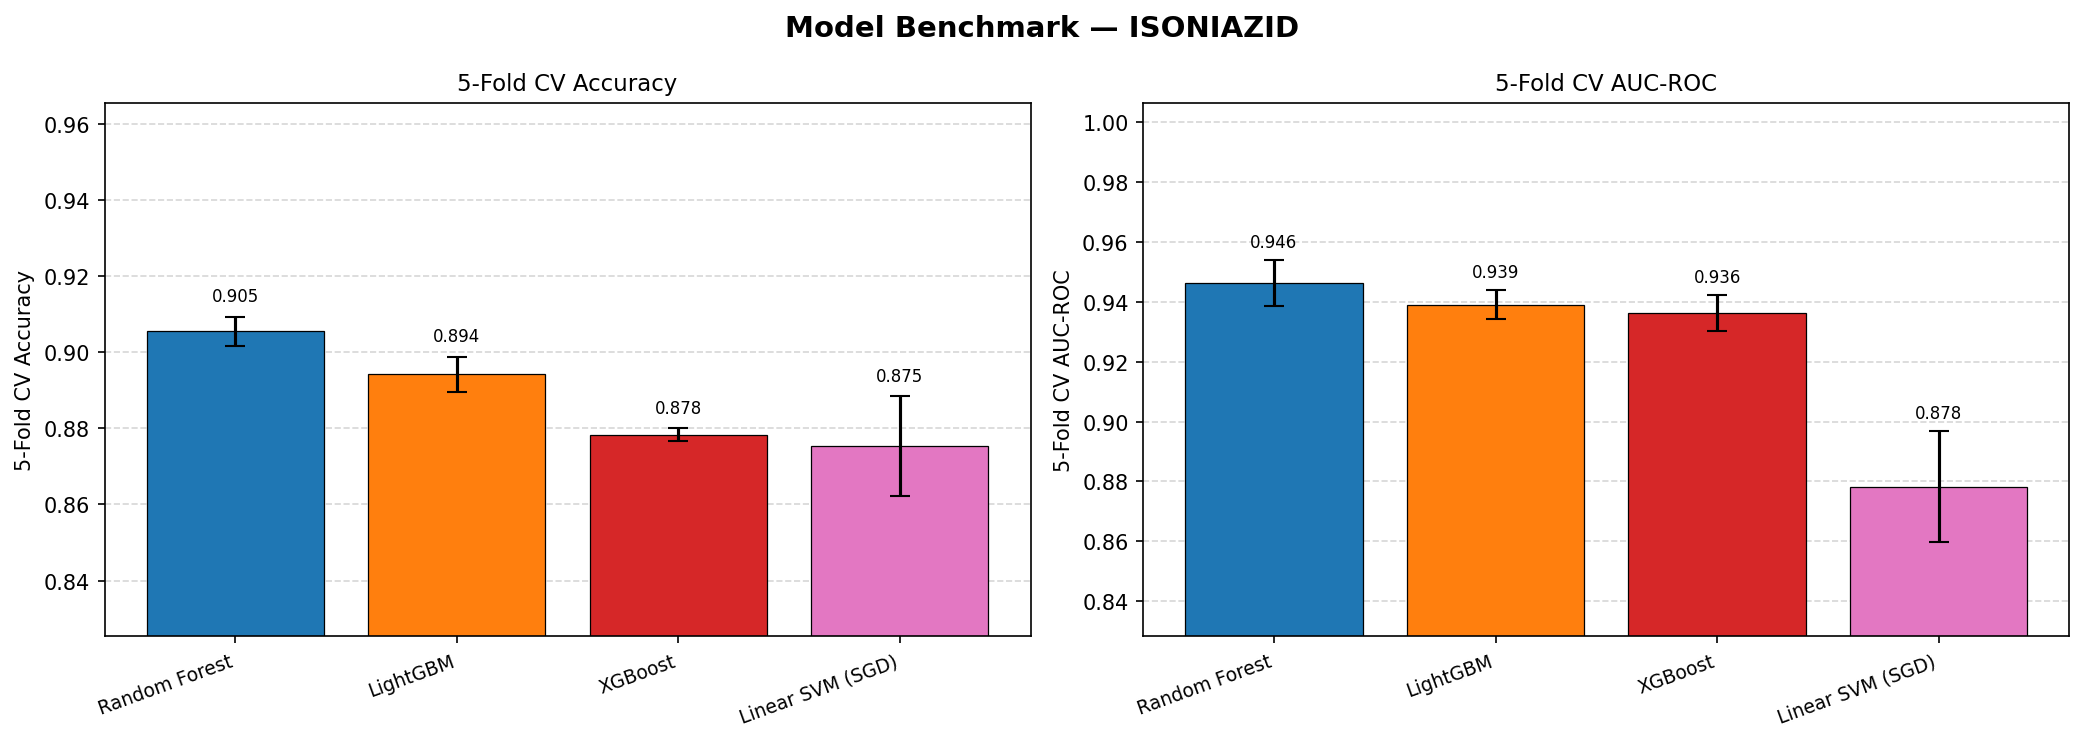
\includegraphics[width=0.85\linewidth]{figures/fig3b_benchmark_isoniazid.png}
\caption{Seven-model CV AUC-ROC comparison for rifampicin (top) and isoniazid (bottom); ethambutol and pyrazinamide follow the same ranking pattern (Random Forest best, linear SVM weakest) per Table~\ref{tab:modelcomparison}.}
\label{fig:benchmark}
\end{figure}

\subsection*{Cross-drug attribution and co-resistance signal}

Because the four drug labels are correlated at the population level (e.g. multidrug-resistant isolates are jointly resistant to rifampicin and isoniazid far more often than expected under independence), we examined whether SHAP attribution for a shared genomic feature shifts between isolates resistant to only one drug versus isolates co-resistant to both. For the rifampicin--isoniazid pair, the dominant rifampicin feature (\emph{rpoB} S450L, pos\_761155) retains a large mean $|\mathrm{SHAP}|$ in the rifampicin model regardless of isoniazid co-resistance status, while several secondary features -- notably the dominant isoniazid feature \emph{katG} S315T (pos\_2155168) -- show a pronounced attribution shift between the single-drug-resistant and co-resistant groups (Table~\ref{tab:crossdrug}). This pattern is consistent with the two mutations reflecting largely independent, drug-specific resistance mechanisms whose co-occurrence in an isolate reflects epidemiological linkage (sequential or concurrent acquisition of MDR-conferring mutations) rather than a shared causal pathway.

\begin{table}[h]
\centering
\caption{Illustrative cross-drug SHAP attribution shift for the rifampicin--isoniazid (RIF--INH) pair: mean $|\mathrm{SHAP}|$ for a shared feature position when isolates are resistant to only one of the two drugs versus co-resistant to both, ranked by the top five positions with the largest attribution shift (max\_abs\_delta).}
\label{tab:crossdrug}
\small
\begin{tabular}{llrrrr}
\toprule
Position & Gene & RIF-only & INH-only & RIF, co-resist. & INH, co-resist. \\
\midrule
pos\_2155168 & katG & 0.026 & 0.239 & 0.011 & 0.122 \\
pos\_761139  & rpoB & 0.120 & 0.002 & 0.040 & 0.002 \\
pos\_761155  & rpoB & 0.289 & 0.023 & 0.271 & 0.018 \\
pos\_761110  & rpoB & 0.052 & 0.011 & 0.065 & 0.008 \\
pos\_2154724 & katG & 0.010 & 0.022 & 0.006 & 0.009 \\
\bottomrule
\end{tabular}

\vspace{4pt}
\footnotesize
The full drug pair yields 41 shared-position rows; the five with the largest attribution shift are shown. pos\_761155 (rpoB S450L) and pos\_2155168 (katG S315T) are the two dominant, independently validated resistance-determining mutations for rifampicin and isoniazid respectively; their recurrence as top-attribution features in each other's models is consistent with population-level co-occurrence of RIF and INH resistance (i.e. MDR-TB) rather than a direct causal cross-drug mechanism.
\end{table}


\subsection*{Multi-label prediction}

Extending Random Forest to jointly predict all four drug labels achieved a macro-averaged AUC-ROC of 0.919 and a Hamming loss of 0.136 (Table~\ref{tab:multilabel}), both consistent with the per-drug AUC-ROC values above. However, subset accuracy -- the fraction of isolates for which all four labels are predicted correctly simultaneously -- was substantially lower at 0.591, reflecting that a single per-drug misclassification anywhere in the four-drug profile counts as a failure under this stricter metric. Random Forest again outperformed LightGBM, XGBoost, and linear SVM on every multi-label metric.

\begin{table}[h]
\centering
\caption{Multi-label (all four RIPE drugs predicted jointly via \texttt{MultiOutputClassifier}) benchmark on the 5{,}180 isolates labelled for all four drugs; plain $K$-fold CV (stratified CV is not defined for multi-label targets).}
\label{tab:multilabel}
\begin{tabular}{lrrr}
\toprule
Model & Hamming Loss $\downarrow$ & Subset Acc. $\uparrow$ & Macro AUC-ROC $\uparrow$ \\
\midrule
Random Forest    & 0.1361 & 0.5907 & 0.9194 \\
LightGBM         & 0.1407 & 0.5753 & 0.9182 \\
XGBoost          & 0.1614 & 0.5106 & 0.9142 \\
Linear SVM (SGD) & 0.1783 & 0.5010 & 0.8282 \\
\bottomrule
\end{tabular}

\vspace{4pt}
\footnotesize
Subset accuracy requires an exact match across all four drug labels simultaneously, a substantially stricter criterion than the per-drug AUC-ROC values in Tables~\ref{tab:perdrug}--\ref{tab:modelcomparison}.
\end{table}


\subsection*{Case study: an MDR-TB isolate}

To illustrate isolate-level interpretability, we applied the trained per-drug models and their SHAP explainers to a held-out demonstration isolate, ERR040120 (Table~\ref{tab:casestudy}). The isolate was predicted resistant to all four drugs, with near-certain probability for rifampicin and isoniazid (both $P=1.000$) driven overwhelmingly by \emph{rpoB} S450L and \emph{katG} S315T respectively, and lower-confidence resistance predictions for ethambutol ($P=0.733$) and pyrazinamide ($P=0.851$) for which no single feature dominates the attribution to the same degree. This isolate and its precomputed explanations are also used as the default "demo mode" input for the public dashboard described below.

\begin{table}[h]
\centering
\caption{Case study: predicted resistance profile for demo isolate ERR040120 (a multidrug-resistant isolate), with its single top-ranked SHAP feature per drug.}
\label{tab:casestudy}
\begin{tabular}{lrll}
\toprule
Drug & $P$(Resistant) & Prediction & Top SHAP feature (gene, SHAP value) \\
\midrule
Rifampicin   & 1.0000 & Resistant & pos\_761155 (rpoB, $+0.2805$) \\
Isoniazid    & 1.0000 & Resistant & pos\_2155168 (katG, $+0.1787$) \\
Ethambutol   & 0.7334 & Resistant & pos\_4247730 (embB, $+0.1480$) \\
Pyrazinamide & 0.8508 & Resistant & pos\_4247730 (embB, $+0.2233$) \\
\bottomrule
\end{tabular}

\vspace{4pt}
\footnotesize
pos\_761155 (rpoB) and pos\_2155168 (katG) correspond to the well-characterized rpoB~S450L and katG~S315T resistance mutations.
\end{table}


\subsection*{Public dashboard}

To make these per-isolate explanations accessible without requiring local computation, we released an interactive Streamlit dashboard, deployed as a public Hugging Face Space. The dashboard supports a demo mode, which loads the precomputed ERR040120 predictions above with no computation required, and a live mode, in which a user-supplied filtered VCF is encoded against the 2{,}693 AMR-gene feature positions, scored using the corresponding per-drug Random Forest model (downloaded from Hugging Face Hub), and explained in real time via \texttt{TreeExplainer}. The dashboard displays a four-drug resistance-profile summary, per-drug SHAP bar charts of the top 20 contributing features, and an expandable table of the underlying mutations, and allows the resulting explanation to be downloaded as JSON.
